\documentclass{beamer}
\usetheme{Warsaw}  %% Themenwahl
\usepackage{beamerthemeshadow}
\usepackage{graphicx}


\title{DIY-Projektvorstellung}
\author{}
\date{\today}

\begin{document}
\maketitle
%\frame{\frametitle{Inhaltsverzeichnis}\tableofcontents} 

\section{Binary Clock - Die Idee}
\frame{\tableofcontents[currentsection]}
\begin{frame}
Die Binary Clock
	%\frametitle{Demotitel 1}	
		\begin{itemize}
			\item zeigt Stunden und Minuten an 		\pause 
			\item soll mit Batterien funktionieren	\pause 
			\item Uhrzeitanzeige \pause
			\begin{itemize}
				\item mit LCD-Display \pause
				\item oder LEDs \pause
			\end{itemize}
			\item nutzt einen Microcontroller
		\end{itemize} 
\end{frame}

\begin{frame}
\begin{figure}[ht]
	\centering
	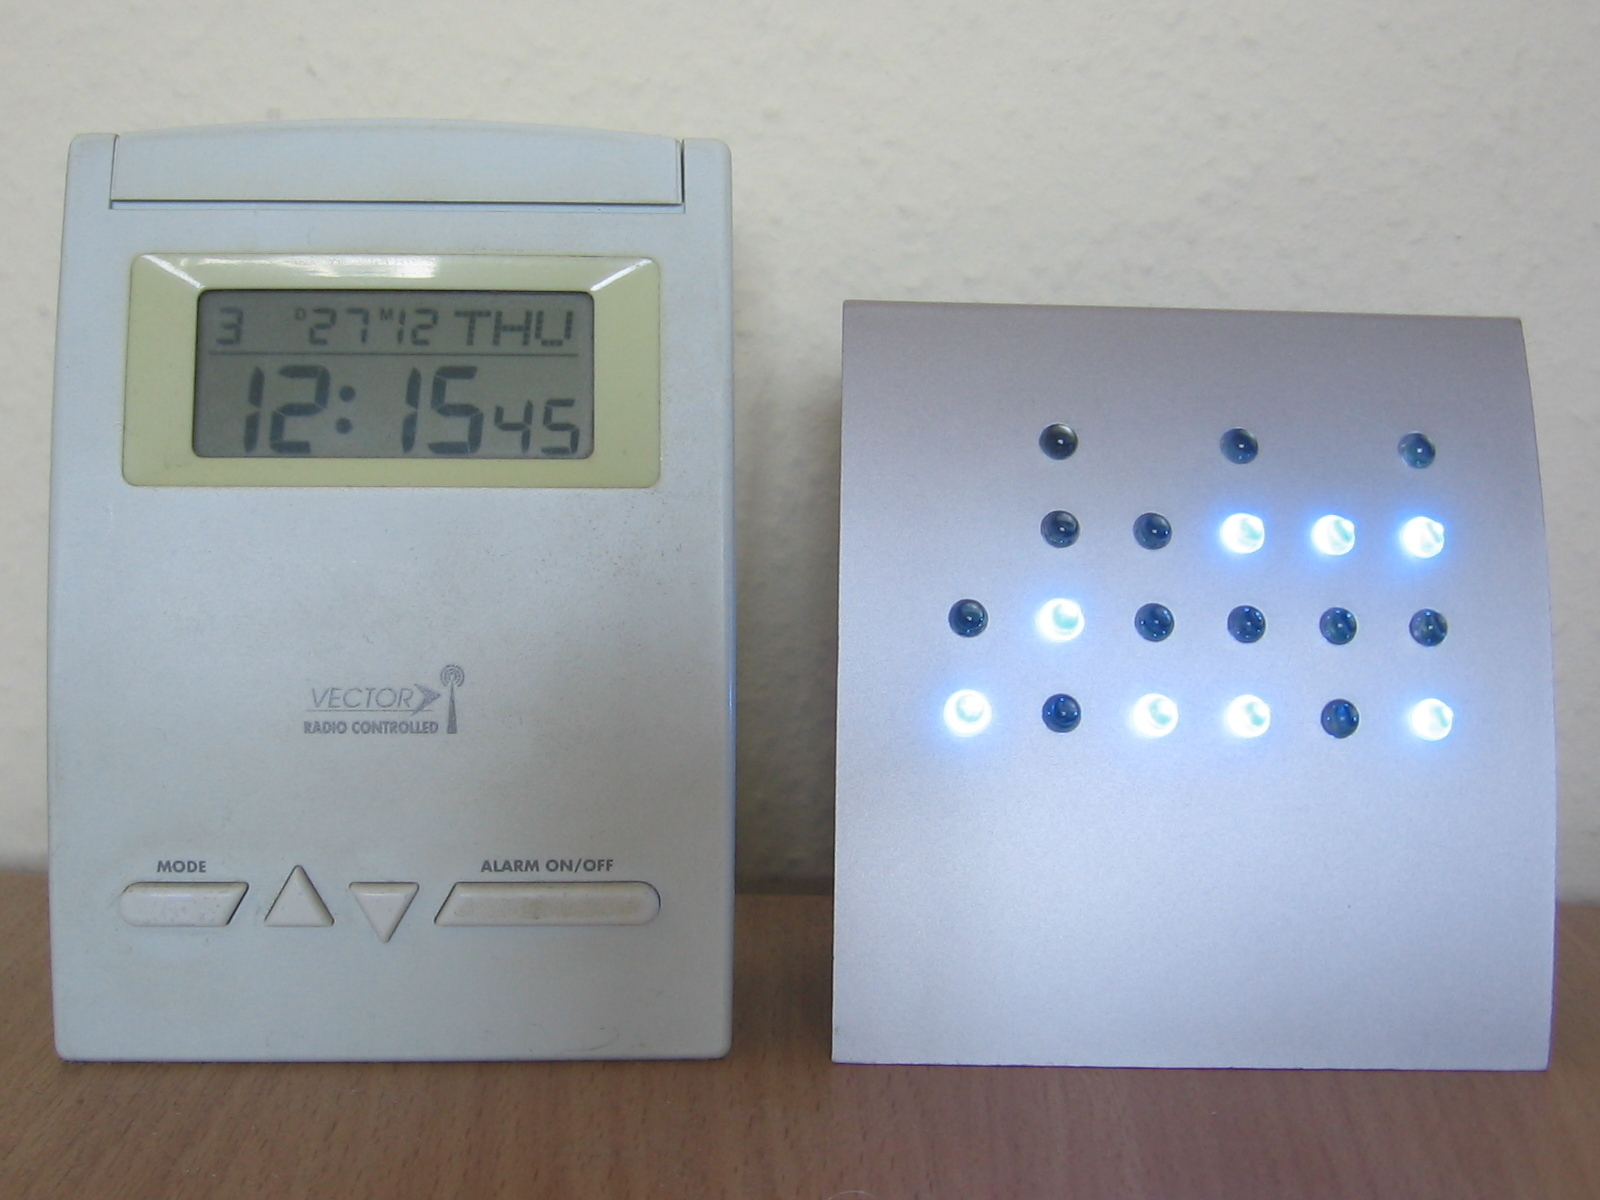
\includegraphics[width=0.7\textwidth]{img/Digital-BCD-clock.jpg}
\end{figure}
\end{frame}


\begin{frame}
	\begin{figure}[ht]
		\centering
		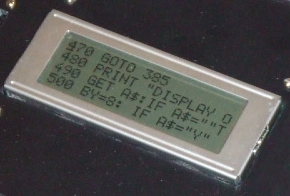
\includegraphics[width=0.7\textwidth]{img/DTV-LCD-MOD.jpg}
	\end{figure}
\end{frame}


\begin{frame}
	\begin{figure}[ht]
		\centering
		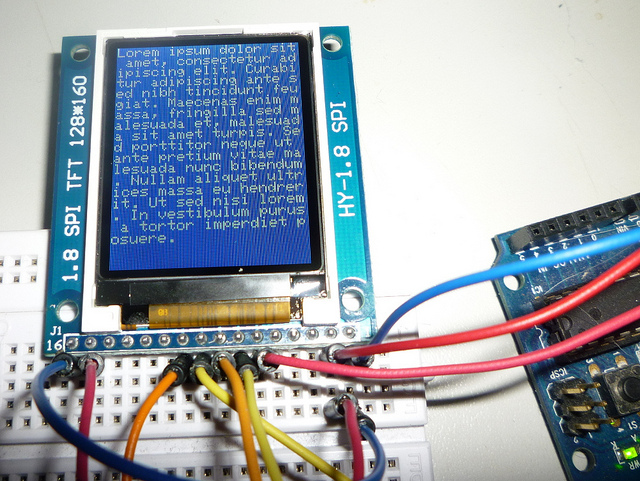
\includegraphics[width=0.7\textwidth]{img/SPI_TFT_LCD_BY_flickr_nathanchantrell.jpg}\footnote{image by flickr.com/photos/nathanchantrell CC BY-NC-ND 2.0} 
	\end{figure}
\end{frame}


\end{document}